\section{Benchmark Design}
\label{sec:benchmark}

\textsc{ui-bench} is specified by four coupled components: the DSL and its
restricted parser, the scene generator, the deterministic renderer, and the
render-based evaluator. We describe each in turn.

\subsection{The ui-bench DSL}
\label{sec:dsl}

A ui-bench program is a sequence of top-level function calls, one per line.
There are exactly four primitive functions:

\begin{lstlisting}
filled_circle(cx=<int>, cy=<int>, radius=<int>)
circle(cx=<int>, cy=<int>, radius=<int>, stroke=<int>)
filled_square(cx=<int>, cy=<int>, size=<int>)
square(cx=<int>, cy=<int>, size=<int>, stroke=<int>)
\end{lstlisting}

The parser is implemented on top of Python's \texttt{ast} module but enforces a
strict whitelist: only top-level expression statements; only calls to the four
whitelisted names; only keyword arguments; only integer literals (including
\texttt{+n}/\texttt{-n} unary forms). Imports, variables, loops, comprehensions,
attribute access, starred arguments, duplicate keywords, and unexpected keywords
are rejected with typed errors. Parameter ranges are validated:
$\texttt{cx},\texttt{cy} \in [0, 511]$; $\texttt{radius},\texttt{size} \in [1, 512]$;
$\texttt{stroke} \in [1, \texttt{radius}]$ for circles and
$\texttt{stroke} \in [1, \lceil \texttt{size}/2 \rceil]$ for squares. Shapes may
extend beyond the canvas and are clipped deterministically at render time.

The serializer is canonical: one call per line, fixed keyword order per
primitive, normalized whitespace, no imports or boilerplate.

\subsection{Renderer}
\label{sec:renderer}

The renderer uses Pillow's \texttt{ImageDraw} to produce a $512 \times 512$
8-bit grayscale image. Backgrounds are white ($255$) and shapes are black ($0$).
\texttt{FilledCircle} uses \texttt{draw.ellipse(fill)}; \texttt{Circle} uses
\texttt{draw.ellipse(outline, width=stroke)}; and the square counterparts use
\texttt{draw.rectangle} with the same conventions. Program order is preserved
in the render loop, but the binary palette makes scenes order-invariant: later
shapes can add foreground pixels but cannot erase them. True order-sensitive
evaluation is deferred to a future version.

\subsection{Generator and Difficulty Tiers}
\label{sec:generator}

The generator is seeded by a single integer and uses only
\texttt{random.Random(seed)} for determinism. Scenes are produced by
rejection-sampling candidate shapes until they satisfy tier-specific constraints
on (i) shape count, (ii) primitive extent (radius or size), (iii) stroke width,
(iv) canvas clipping probability, and (v) the maximum allowed bounding-box IoU
between the new shape and any existing shape. A tier may additionally require at
least one pairwise bounding-box overlap.

\begin{table}[t]
  \centering
  \small
  \begin{tabular}{lcccccc}
  \toprule
  Tier & \# shapes & Extent & Stroke & Clip prob. & Max bbox IoU & Overlap? \\
  \midrule
  Easy & $1$--$3$ & $[64, 160]$ & $[2, 6]$ & $0.00$ & $0.02$ & no \\
  Medium & $3$--$6$ & $[32, 128]$ & $[2, 8]$ & $0.25$ & $0.35$ & no \\
  Hard & $6$--$10$ & $[16, 128]$ & $[1, 10]$ & $1.00$ & $-$ & yes \\
  \bottomrule
  \end{tabular}
  \caption{Difficulty tiers used to structure generation in \textsc{ui-bench}. ``Extent'' is the radius or size range;
  a missing Max bbox IoU indicates no constraint.}
  \label{tab:difficulty-tiers}
\end{table}

Each generated sample is written to disk as a PNG together with a JSON metadata
file containing the sample ID, split, difficulty, seed, canvas size, shape count,
shape inventory, ground-truth program, and render configuration. Our frozen
evaluation split \textsc{eval\_v1} uses contiguous seeds $0{-}49$ per tier,
yielding 150 samples total; their SHA-256 hashes are published alongside the
dataset.

\begin{figure}[t]
  \centering
  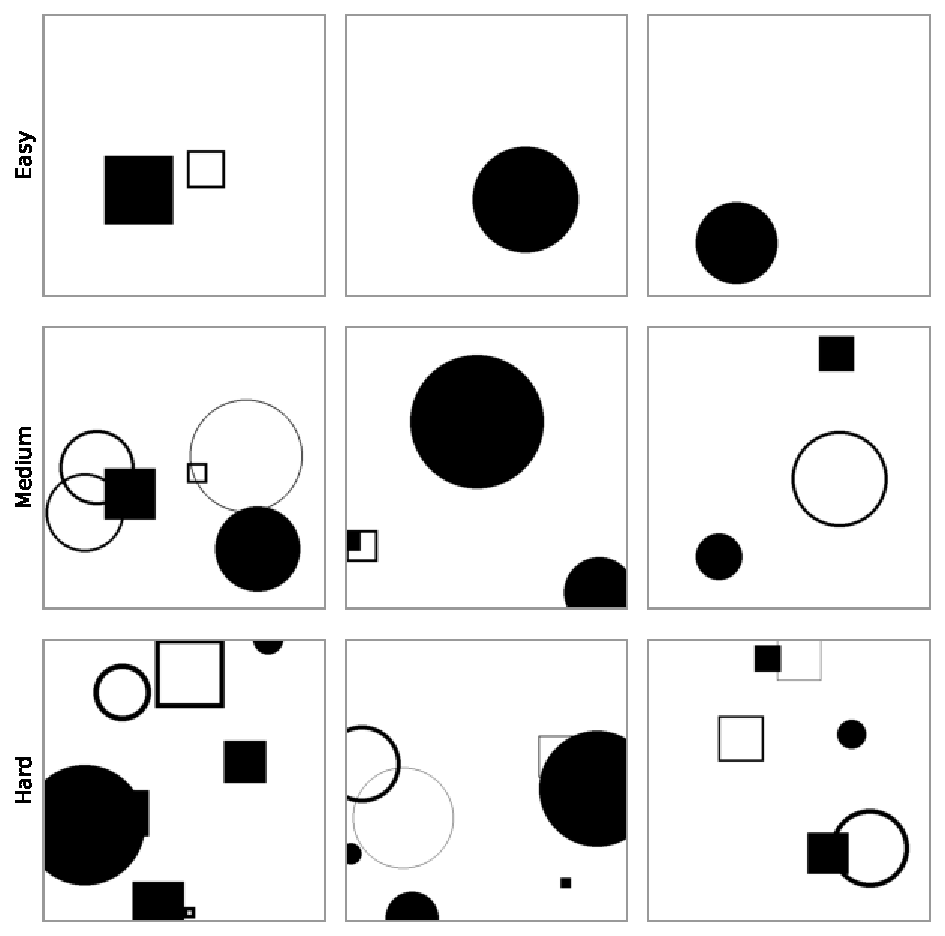
\includegraphics[width=0.85\linewidth]{figures/fig_sample_grid.pdf}
  \caption{Representative samples from \textsc{eval\_v1} at each difficulty
  tier. The three tiers differ in shape count, extent, and overlap.}
  \label{fig:sample-grid}
\end{figure}

\subsection{Evaluator}
\label{sec:evaluator}

Given a target image $I_t$ and a predicted DSL program $p$, the evaluator
attempts to parse $p$ through the restricted parser, render the resulting scene
into $I_p$, and compare rasters. We report five metrics.

\begin{itemize}
  \item \textbf{Exact match} -- $1$ if $I_t = I_p$ pixel-exactly, else $0$.
  \item \textbf{Pixel accuracy} -- fraction of pixels equal between $I_t$ and $I_p$.
  \item \textbf{Foreground IoU} -- intersection-over-union of black pixels
    between $I_t$ and $I_p$ (convention: if both sets are empty, IoU is $1$).
  \item \textbf{Parse success} -- $1$ if the parser accepts $p$, else $0$.
  \item \textbf{Execution success} -- $1$ if rendering the parsed scene succeeds, else $0$.
\end{itemize}

On parse or execution failure, all similarity metrics fall to $0$ and the
failure type is recorded for later analysis. We aggregate metrics over the full
split and also report per-tier breakdowns.
